\subsubsection{Gate-Treiber, H-Brücke und BLDC}
\label{subsubsec:Inbetriebnahme_Gate_Treiber}

Der Gate-Treiber wird mit einem Testprogramm in Betrieb genommen. Das Programm initialisiert die benötigte Hardware des Mikrocontrollers (UART, SPI, Pins), enthält die Library des FOC- und Gate-Treibers und ermöglicht das Debugen über die serielle Schnittstelle. Die Software TMCL-IDE hilft bei der Bestimmung der Parameter für den Gate-Treiber. Welche Register wie beschrieben wurden ist im Anhang Kapitel \ref{Appendix:TMC6200_Register} zu sehen. Die Initialisierung sowie das Auslesen gewisser Register ist ebenfalls mit der Testapplikation ''\textit{3\underline{ }Motor\underline{ }Openloop}'' möglich. Dazu müssen einige Zeilen auskommentiert werden.

Es wird erwartet, dass die Gate-CTRL-Signale vom Gate-Treiber aufbereitet werden und eine Spannung an den High- und Lowside-MOSFETs anliegt und die H-Brücke den Motor steuert.

\paragraph{Setup}\mbox{}

\begin{figure}[H]
	\centering
	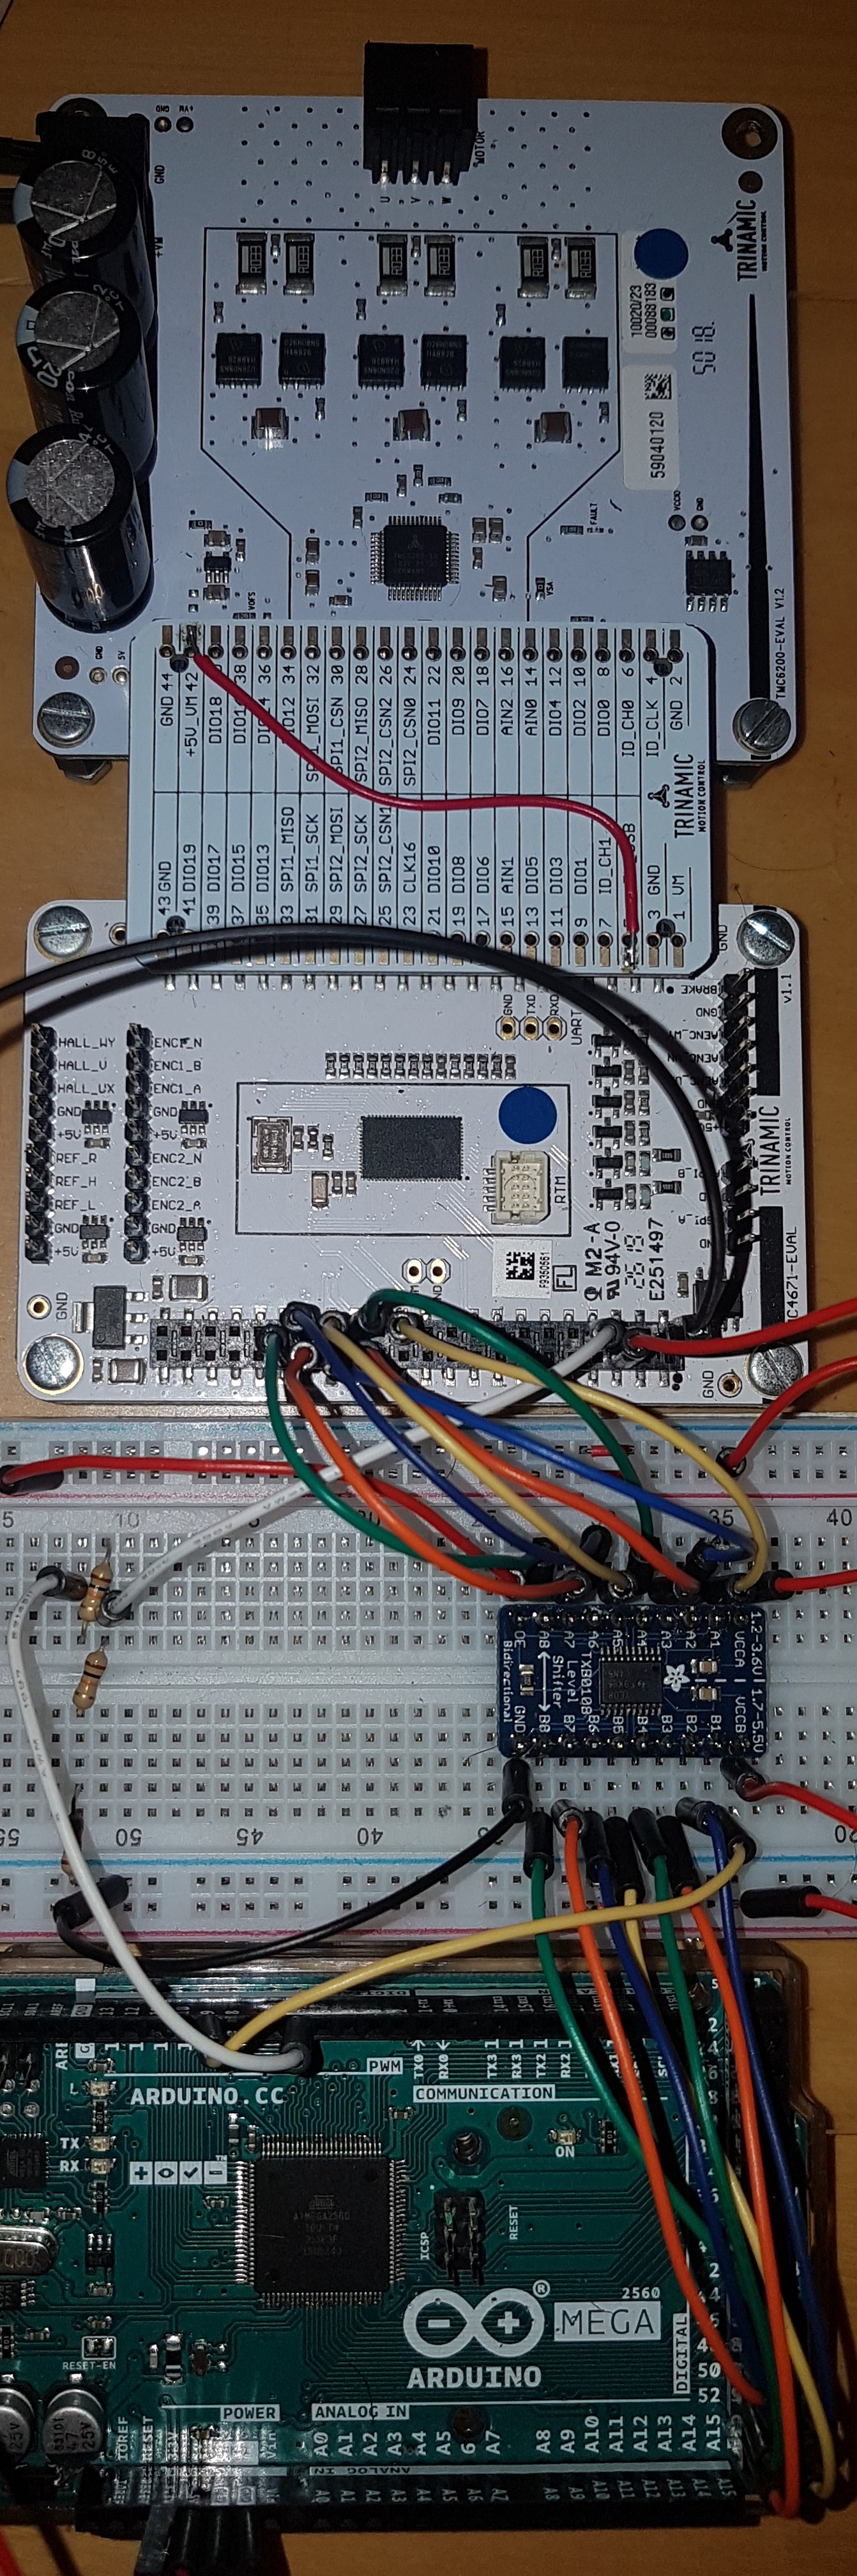
\includegraphics[angle=270,width=\textwidth]{graphics/2_komplett1}
	\caption{Gesamtansicht Setup.}
	\label{fig:2_komplett1}
\end{figure}

\textbf{Achtung}, wenn die Scripts auf den Mikrocontroller des PartyMixers geladen werden ist darauf zu achten, dass die Achse des Motors frei beweglich ist und das Förderband nicht mit der Achse mitdreht, da ansonsten Schäden an der Maschine entstehen können. Es wird empfohlen die Scripts mit Mikrocontroller und EVAL-Boards zu testen.

Vorgehen:
\begin{enumerate}
\item Benötigte Applikation, welche im Software-Ordner auf dem USB-Stick oder Github \cite{aebi_projekt-6softwareatmega_2020} zu finden ist, in Atmel Studio öffnen.\\
\textcolor{magenta}{Software\textrightarrow Atmega\textrightarrow 3\underline{ }Motor\underline{ }Openloop\textrightarrow 1\underline{ }Motor\underline{ }Testsoftware\textrightarrow Motor}\\


\item Software anpassen:\\
\textcolor{OliveGreen}{
	initTMC6200;\\
	initTMC4671\underline{ }Openloop();\\
\\
    while (1) \\
    \{\\
		\underline{ }delay\underline{ }ms(5000);\\
		read\underline{ }registers\underline{ }TMC6200();\\
		\underline{ }delay\underline{ }ms(10000);\\
		read\underline{ }registers\underline{ }TMC4671();\\
    \}
}\newline
\item Software hochladen:\\
\textcolor{blue}{AtmelStudio\textrightarrow Tools\textrightarrow PartyMixer}\\
\end{enumerate}

Ergebnis: Die Gate-CTRL-Signale liegen an. Abbildung \ref{fig:TMC6200_Gate_Signal_H} zeigt die High-Side-Gatesignale, Abbildung \ref{fig:TMC6200_Gate_Signal_L} die Low-Side-Gatesignale. Sie führen auf die MOSFET-Gates, welche die H-Brücke bilden und den Leistungsteil schalten.

\begin{figure}[H]
\center
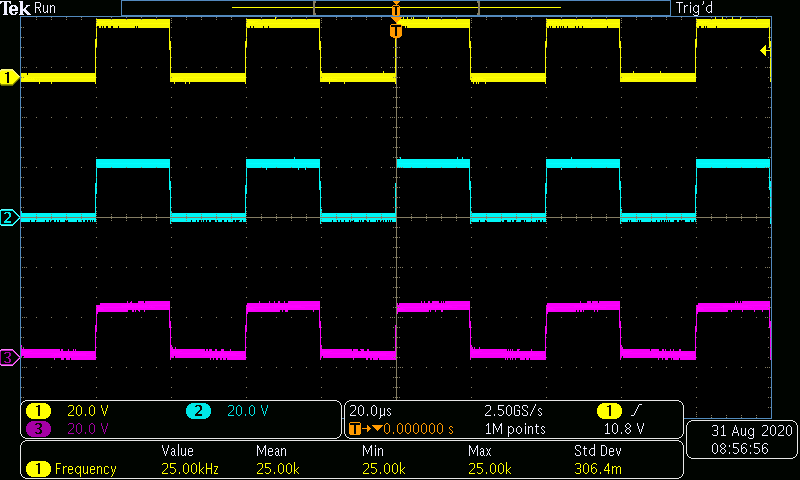
\includegraphics[width = 0.8\textwidth]{graphics/TMC6200_Gate_Signal_H}
\caption{High-Side-Gatesignale von Gate-Treiber auf H-Brücke. Gelb = U, Blau = V, Magenta = W}
\label{fig:TMC6200_Gate_Signal_H}
\end{figure}

\begin{figure}[H]
\center
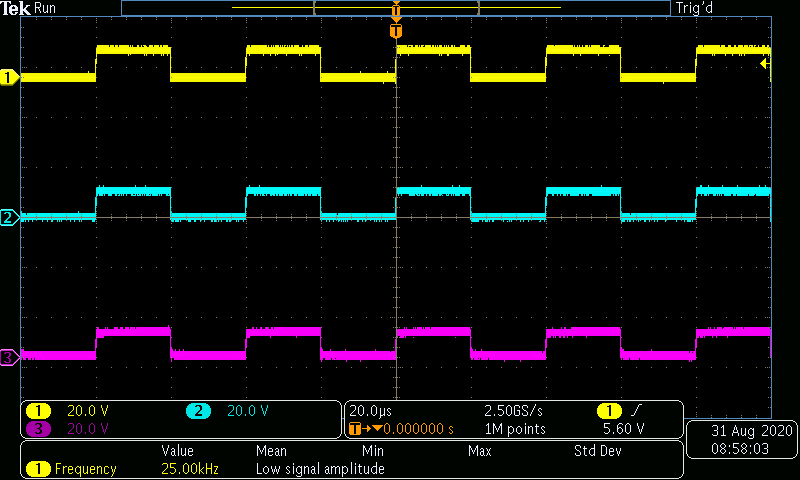
\includegraphics[width = 0.8\textwidth]{graphics/TMC6200_Gate_Signal_L}
\caption{Low-Side-Gatesignale von Gate-Treiber auf H-Brücke. Gelb = U, Blau = V, Magenta = W}
\label{fig:TMC6200_Gate_Signal_L}
\end{figure}
\newpage
Die Abbildung \ref{fig:OpenLoop_TestDrive2} zeigt die Schaltsignale am Ausgang der H-Brücke.

\begin{figure}[H]
	\centering
	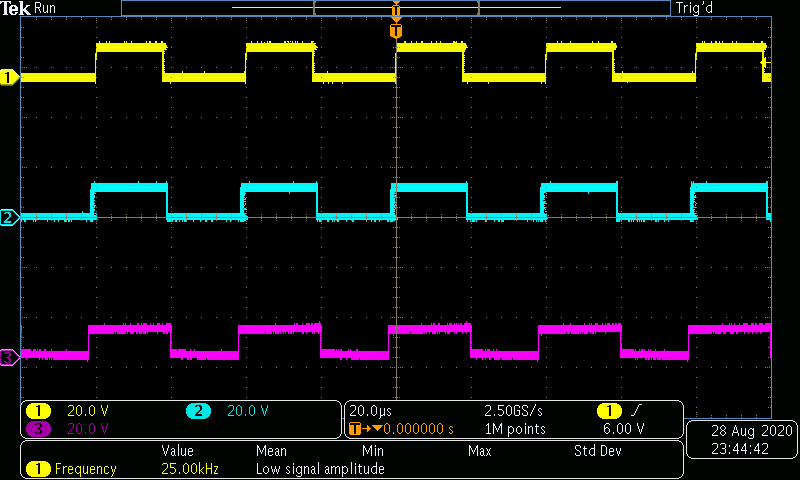
\includegraphics[width=0.8\textwidth]{graphics/OpenLoop_TestDrive2}
	\caption{Schaltsignale während dem Openloop Testdrive. Gelb = U, Blau = V, Magenta = W}
	\label{fig:OpenLoop_TestDrive2}
\end{figure}

Wird der Motor angeschlossen und der Mikrocontroller neu gestartet, der Motor sich mit der vorgegebenen Open-Loop-Geschwindigkeit.